% !TeX program = lualatex
% Compile: lualatex -interaction=nonstopmode -halt-on-error Guia_ilustrado_do_codigo.tex
\documentclass[10pt,a4paper]{article}
\usepackage{iftex}
\ifLuaTeX\else\errmessage{Este documento requer LuaLaTeX}\fi
\usepackage{amsmath}
\usepackage{fontspec}
\setmainfont{TeX Gyre Heros}
\setmonofont{Latin Modern Mono}[Scale=0.87]
\usepackage[margin=17mm,top=15mm,bottom=19mm]{geometry}
\usepackage{xcolor}
\definecolor{navy}{HTML}{142D4E}
\definecolor{teal}{HTML}{008878}
\definecolor{pale}{HTML}{EDF5F7}
\usepackage{tikz}
\usetikzlibrary{arrows.meta,positioning}
\usepackage[most]{tcolorbox}
\usepackage{fancyvrb}
\usepackage{fancyhdr}
\usepackage{microtype}
\usepackage{hyperref}
\hypersetup{colorlinks=true,urlcolor=teal,pdftitle={Guia ilustrado do código},pdfauthor={}}
\pagestyle{fancy}\fancyhf{}
\fancyfoot[L]{\scriptsize Experimento corrigido | 14/10/2026 | Guia do código existente}
\fancyfoot[R]{\scriptsize\thepage / 8}
\renewcommand{\headrulewidth}{0pt}
\setlength{\parindent}{0pt}\setlength{\parskip}{7pt}
\setlength{\emergencystretch}{3em}
\color{navy}
\newcommand{\blocktitle}[1]{\par\vspace{3pt}{\large\bfseries\color{teal}#1}\par}
\newenvironment{codebox}{\VerbatimEnvironment\begin{tcolorbox}[colback=pale,colframe=pale,boxrule=0pt,arc=2mm,left=2mm,right=2mm,top=1mm,bottom=1mm]\begin{Verbatim}[fontsize=\small]}{\end{Verbatim}\end{tcolorbox}}
\begin{document}
\begin{tcolorbox}[colback=navy,colframe=navy,arc=2mm,boxrule=0pt,left=4mm,right=4mm,top=4mm,bottom=4mm]
{\color{white}\small 01 | Mapa do projeto\par\medskip\fontsize{23}{27}\selectfont\bfseries O que o programa faz\par\medskip\normalfont\small Quatro modelos, quatro condições e resultados separados por execução.}\end{tcolorbox}
\begin{center}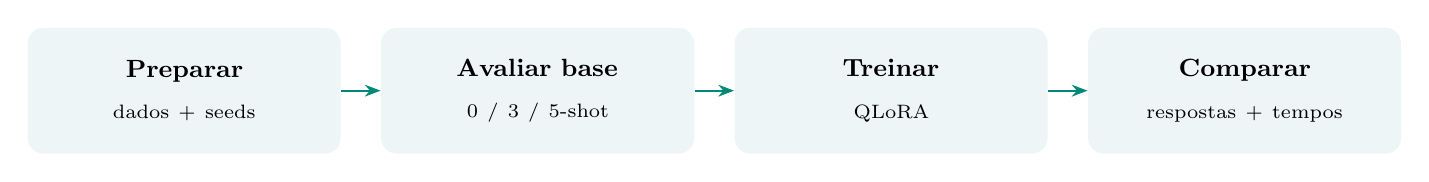
\begin{tikzpicture}[box/.style={fill=pale,rounded corners=2mm,minimum height=16mm,inner sep=2mm,align=center,text width=35.75mm},arr/.style={-{Stealth[length=2mm]},teal,thick}]
\node[box] (n0) {\small\bfseries Preparar\\[3pt]\normalfont\scriptsize dados + seeds};
\node[right=5mm of n0,box] (n1) {\small\bfseries Avaliar base\\[3pt]\normalfont\scriptsize 0 / 3 / 5-shot};
\draw[arr] (n0.east) -- (n1.west);
\node[right=5mm of n1,box] (n2) {\small\bfseries Treinar\\[3pt]\normalfont\scriptsize QLoRA};
\draw[arr] (n1.east) -- (n2.west);
\node[right=5mm of n2,box] (n3) {\small\bfseries Comparar\\[3pt]\normalfont\scriptsize respostas + tempos};
\draw[arr] (n2.east) -- (n3.west);
\end{tikzpicture}\end{center}
O programa compara modelos antes de qualquer ajuste com uma versão ajustada por fine-tuning. Os exemplos de few-shot entram no prompt. Somente a condição \textbf{fine-tuned} treina adaptadores.

\blocktitle{Bloco A - Quem organiza tudo}
\textbf{rodar\_todos.py}: escolhe modelos, seeds e repetições; abre um processo por trial e aguarda seu término. Um trial é uma execução completa de um modelo com uma seed e uma repetição.

\blocktitle{Bloco B - Quem executa o experimento}
\textbf{modelos/gemma4.py, huatuogpt.py, medgemma.py e qwen35.py}: carregam dados e modelo, montam prompts, treinam quando necessário e avaliam as quatro condições. Este guia usa os nomes de funções comuns aos scripts.

\blocktitle{Bloco C - Quem prepara e registra}
\textbf{prompts\_medicos.py} define a persona e lê seeds. \textbf{registro.py} grava logs, tabelas e ambiente. \textbf{consolidar.py} reúne execuções concluídas. \textbf{resumir.py} calcula resumos entre execuções.

\begin{codebox}
CONDITIONS = [('zero-shot', 0, False),
              ('3-shot', 3, False),
              ('5-shot', 5, False),
              ('fine-tuned', 0, True)]
\end{codebox}
Leia cada tupla como: \textbf{nome da condição, número de exemplos, deve treinar?} O modelo original é recarregado a cada condição.

\newpage
\begin{tcolorbox}[colback=navy,colframe=navy,arc=2mm,boxrule=0pt,left=4mm,right=4mm,top=4mm,bottom=4mm]
{\color{white}\small 02 | Executor\par\medskip\fontsize{23}{27}\selectfont\bfseries Um modelo por vez\par\medskip\normalfont\small Arquivo: rodar\_todos.py | Função principal: main()}\end{tcolorbox}
\begin{center}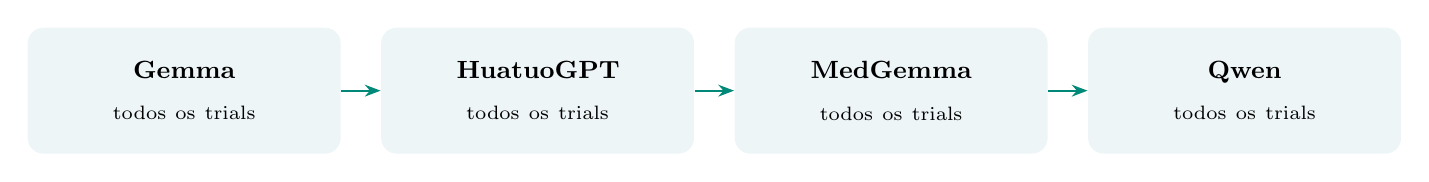
\begin{tikzpicture}[box/.style={fill=pale,rounded corners=2mm,minimum height=16mm,inner sep=2mm,align=center,text width=35.75mm},arr/.style={-{Stealth[length=2mm]},teal,thick}]
\node[box] (n0) {\small\bfseries Gemma\\[3pt]\normalfont\scriptsize todos os trials};
\node[right=5mm of n0,box] (n1) {\small\bfseries HuatuoGPT\\[3pt]\normalfont\scriptsize todos os trials};
\draw[arr] (n0.east) -- (n1.west);
\node[right=5mm of n1,box] (n2) {\small\bfseries MedGemma\\[3pt]\normalfont\scriptsize todos os trials};
\draw[arr] (n1.east) -- (n2.west);
\node[right=5mm of n2,box] (n3) {\small\bfseries Qwen\\[3pt]\normalfont\scriptsize todos os trials};
\draw[arr] (n2.east) -- (n3.west);
\end{tikzpicture}\end{center}
A ordem padrão é gemma4 \ensuremath{\rightarrow} huatuogpt \ensuremath{\rightarrow} medgemma \ensuremath{\rightarrow} qwen35. O executor termina todas as seeds e repetições de um modelo antes de iniciar o seguinte. A opção \textbf{--modelos} permite escolher a ordem.

\begin{codebox}
for model in args.modelos:
    for seed in args.seeds:
        for repeticao_seed in range(1, args.repeticoes + 1):
            ...
# Depois, cada processo é iniciado e aguardado:
code = process.wait()
\end{codebox}
O trecho abreviado mostra a ordem real dos laços. Não existe execução paralela de LLMs nesse executor. Ao terminar o processo, seus recursos são liberados; isso evita a competição entre os modelos da campanha, mas não impede outros programas de usarem a GPU.

\blocktitle{Seed não é a mesma coisa que repetição}
\textbf{--seeds 42 123}: muda o sorteio das demonstrações e a aleatoriedade do treino. \textbf{--split-seed 42}: mantém a divisão e a seleção dos dados. \textbf{--repeticoes 2}: executa duas vezes cada seed, inclusive repetindo o fine-tuning.

\begin{center}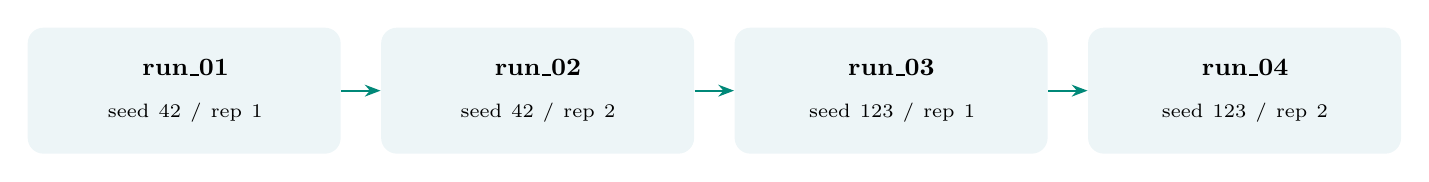
\begin{tikzpicture}[box/.style={fill=pale,rounded corners=2mm,minimum height=16mm,inner sep=2mm,align=center,text width=35.75mm},arr/.style={-{Stealth[length=2mm]},teal,thick}]
\node[box] (n0) {\small\bfseries run\_01\\[3pt]\normalfont\scriptsize seed 42 / rep 1};
\node[right=5mm of n0,box] (n1) {\small\bfseries run\_02\\[3pt]\normalfont\scriptsize seed 42 / rep 2};
\draw[arr] (n0.east) -- (n1.west);
\node[right=5mm of n1,box] (n2) {\small\bfseries run\_03\\[3pt]\normalfont\scriptsize seed 123 / rep 1};
\draw[arr] (n1.east) -- (n2.west);
\node[right=5mm of n2,box] (n3) {\small\bfseries run\_04\\[3pt]\normalfont\scriptsize seed 123 / rep 2};
\draw[arr] (n2.east) -- (n3.west);
\end{tikzpicture}\end{center}
\textbf{Na prática:} Esses quatro trials são concluídos para Gemma antes de começar HuatuoGPT. A seed aparece no terminal e em status.json. Nos CSVs consolidados, procure exec\_seed.

Se um processo falhar, a campanha para e salva o log. \textbf{--retomar} pula apenas trials completos com código e configuração iguais; não continua um treino interrompido.

\newpage
\begin{tcolorbox}[colback=navy,colframe=navy,arc=2mm,boxrule=0pt,left=4mm,right=4mm,top=4mm,bottom=4mm]
{\color{white}\small 03 | Preparação dos dados\par\medskip\fontsize{23}{27}\selectfont\bfseries Treino e teste separados\par\medskip\normalfont\small Bloco de datasets | make\_demo\_pool()}\end{tcolorbox}
\begin{center}
\begin{tikzpicture}[box/.style={fill=pale,rounded corners=2mm,minimum height=16mm,inner sep=2mm,align=center,text width=50.666666666666664mm},arr/.style={-{Stealth[length=2mm]},teal,thick}]
\node[box] (n0) {\small\bfseries MedQuAD\\[3pt]\normalfont\scriptsize 240 itens filtrados};
\node[right=5mm of n0,box] (n1) {\small\bfseries Treino\\[3pt]\normalfont\scriptsize 192 exemplos};
\draw[arr] (n0.east) -- (n1.west);
\node[right=5mm of n1,box] (n2) {\small\bfseries Teste\\[3pt]\normalfont\scriptsize 48 exemplos};
\draw[arr] (n1.east) -- (n2.west);
\end{tikzpicture}\end{center}
O script filtra respostas e perguntas, remove perguntas idênticas após normalização, seleciona 240 exemplos e separa 192 para treino e 48 para avaliação. As primeiras 20 perguntas do teste também são usadas no bloco de velocidade.

\blocktitle{Cada conjunto tem uma função}
\textbf{MedQuAD:} respostas abertas; fornece o treino do fine-tuning, as referências para avaliação textual e as demonstrações de sua própria tarefa.

\textbf{MedQA:} até 100 perguntas do split oficial de teste, com quatro alternativas. As demonstrações vêm do split de treino. Não é usado como treino do fine-tuning neste código.

\textbf{PubMedQA:} até 100 itens de pqa\_labeled são reservados para avaliação; o restante fica disponível para demonstrações. É uma divisão própria do experimento, não o teste oficial completo. Também não treina o adaptador.

\begin{codebox}
train_dataset, eval_dataset = split_dataset['train'], \
                              split_dataset['test']
# Na condição fine-tuned:
train_regime(model, train_dataset, 5, condition)
\end{codebox}
\blocktitle{O que a proteção contra vazamento faz}
\textbf{make\_demo\_pool()} exclui perguntas do teste com texto normalizado igual e remove duplicatas no conjunto de demonstrações. A resposta da pergunta avaliada não é inserida como exemplo.

\textbf{Na prática:} Os exemplos few-shot atuais vêm dos datasets, não de perguntas buscadas na internet. As personas foram adaptadas de referências públicas. A filtragem não verifica paráfrases, sobreposição entre datasets ou dados de pré-treinamento.

\newpage
\begin{tcolorbox}[colback=navy,colframe=navy,arc=2mm,boxrule=0pt,left=4mm,right=4mm,top=4mm,bottom=4mm]
{\color{white}\small 04 | Construção do prompt\par\medskip\fontsize{23}{27}\selectfont\bfseries Onde entram os 3 ou 5 shots\par\medskip\normalfont\small select\_demonstrations() \ensuremath{\rightarrow} make\_messages() \ensuremath{\rightarrow} build\_prompt()}\end{tcolorbox}
\begin{center}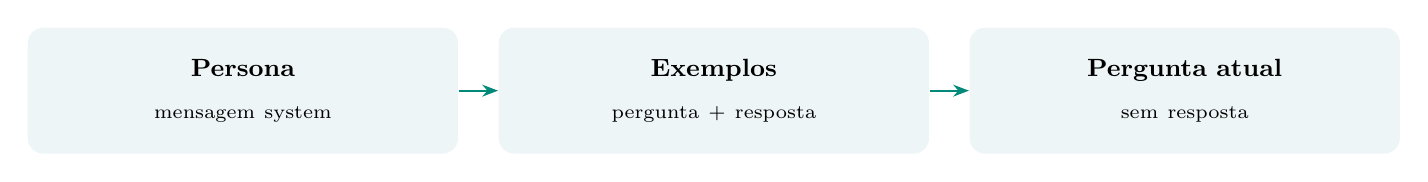
\begin{tikzpicture}[box/.style={fill=pale,rounded corners=2mm,minimum height=16mm,inner sep=2mm,align=center,text width=50.666666666666664mm},arr/.style={-{Stealth[length=2mm]},teal,thick}]
\node[box] (n0) {\small\bfseries Persona\\[3pt]\normalfont\scriptsize mensagem system};
\node[right=5mm of n0,box] (n1) {\small\bfseries Exemplos\\[3pt]\normalfont\scriptsize pergunta + resposta};
\draw[arr] (n0.east) -- (n1.west);
\node[right=5mm of n1,box] (n2) {\small\bfseries Pergunta atual\\[3pt]\normalfont\scriptsize sem resposta};
\draw[arr] (n1.east) -- (n2.west);
\end{tikzpicture}\end{center}
A persona descreve a perspectiva desejada: clínico ou pesquisador biomédico. Ela não conta como shot. Um shot é um par completo de \textbf{pergunta e resposta de demonstração}. A persona é mantida entre as condições.

\begin{codebox}
messages = [{'role': 'system', 'content': system_prompt}]
for demo in demos:
    messages.extend([
        {'role': 'user', 'content': demo['user']},
        {'role': 'assistant', 'content': demo['assistant']}
    ])
messages.append({'role': 'user', 'content': user_text})
\end{codebox}
\blocktitle{Como a seleção permanece reproduzível}
A função combina \textbf{seed + tarefa + pergunta} em um hash. Esse valor inicializa o sorteio de cinco exemplos. O 3-shot usa os primeiros três dos mesmos cinco usados pelo 5-shot. A pergunta avaliada permanece igual entre as condições.

\begin{center}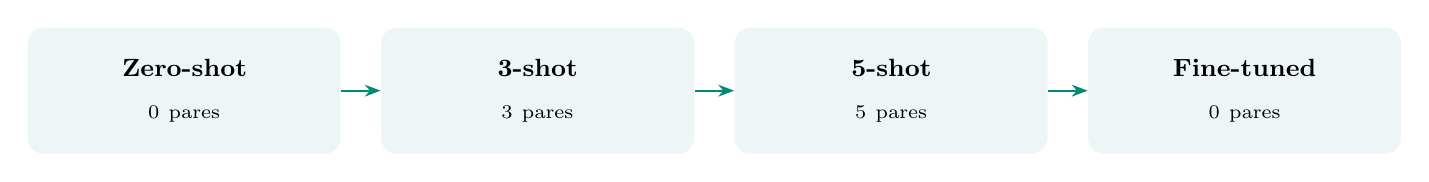
\begin{tikzpicture}[box/.style={fill=pale,rounded corners=2mm,minimum height=16mm,inner sep=2mm,align=center,text width=35.75mm},arr/.style={-{Stealth[length=2mm]},teal,thick}]
\node[box] (n0) {\small\bfseries Zero-shot\\[3pt]\normalfont\scriptsize 0 pares};
\node[right=5mm of n0,box] (n1) {\small\bfseries 3-shot\\[3pt]\normalfont\scriptsize 3 pares};
\draw[arr] (n0.east) -- (n1.west);
\node[right=5mm of n1,box] (n2) {\small\bfseries 5-shot\\[3pt]\normalfont\scriptsize 5 pares};
\draw[arr] (n1.east) -- (n2.west);
\node[right=5mm of n2,box] (n3) {\small\bfseries Fine-tuned\\[3pt]\normalfont\scriptsize 0 pares};
\draw[arr] (n2.east) -- (n3.west);
\end{tikzpicture}\end{center}
\textbf{apply\_chat\_template()} transforma as mensagens no formato do modelo. \textbf{encode\_prompt()} converte o texto em IDs de tokens e reserva espaço para a resposta. Se ultrapassar o limite de contexto configurado, o código gera erro em vez de cortar os exemplos silenciosamente.

\textbf{Na prática:} Para ver o prompt efetivamente montado, abra registros/prompts.csv: messages contém as mensagens, demo\_ids identifica os exemplos e seed informa o sorteio. Pedir uma persona não garante correção médica.

\newpage
\begin{tcolorbox}[colback=navy,colframe=navy,arc=2mm,boxrule=0pt,left=4mm,right=4mm,top=4mm,bottom=4mm]
{\color{white}\small 05 | Modelo e treinamento\par\medskip\fontsize{23}{27}\selectfont\bfseries O que o QLoRA altera\par\medskip\normalfont\small build\_model() e train\_regime()}\end{tcolorbox}
\begin{center}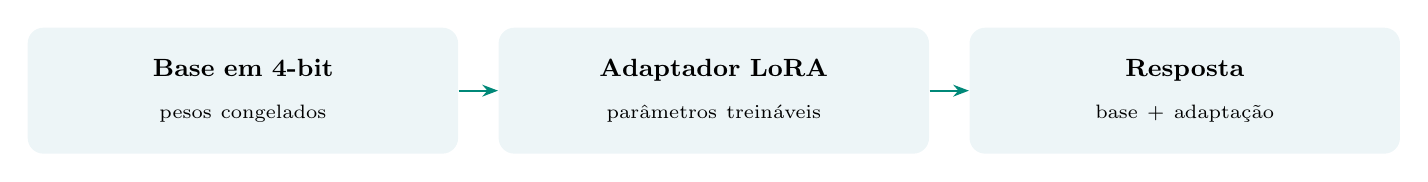
\begin{tikzpicture}[box/.style={fill=pale,rounded corners=2mm,minimum height=16mm,inner sep=2mm,align=center,text width=50.666666666666664mm},arr/.style={-{Stealth[length=2mm]},teal,thick}]
\node[box] (n0) {\small\bfseries Base em 4-bit\\[3pt]\normalfont\scriptsize pesos congelados};
\node[right=5mm of n0,box] (n1) {\small\bfseries Adaptador LoRA\\[3pt]\normalfont\scriptsize parâmetros treináveis};
\draw[arr] (n0.east) -- (n1.west);
\node[right=5mm of n1,box] (n2) {\small\bfseries Resposta\\[3pt]\normalfont\scriptsize base + adaptação};
\draw[arr] (n1.east) -- (n2.west);
\end{tikzpicture}\end{center}
Todos os braços carregam a base com \textbf{load\_in\_4bit=True}. Só o braço fine-tuned adiciona adaptadores LoRA. Treinar adaptadores sobre uma base quantizada é a abordagem QLoRA usada aqui.

\begin{codebox}
load_in_4bit=LOAD_IN_4BIT, full_finetuning=False
# Adaptador da condição fine-tuned:
r=8, lora_alpha=16, lora_dropout=0
# Treinamento:
num_train_epochs=5
learning_rate=2e-5
per_device_train_batch_size=2
gradient_accumulation_steps=16
optim="adamw_torch"
\end{codebox}
O rank 8 define o tamanho da adaptação; alpha 16 controla sua escala. São cinco passagens pelos 192 exemplos. O batch efetivo é \textbf{2 \ensuremath{\times} 16 = 32} em uma GPU: acumula gradientes de 16 microbatches antes de atualizar os parâmetros.

\blocktitle{Não existe merge explícito neste pacote}
O modelo é avaliado com o adaptador ativo e salvo com \textbf{model.save\_pretrained()}. Não há chamada a merge\_and\_unload(). Portanto, os tempos incluem a execução da configuração base quantizada + adaptador.

\begin{codebox}
Sem merge: y = W x + (alpha/r) B(Ax)
Com merge: W' = W + (alpha/r) BA; y = W' x
\end{codebox}
A segunda linha é apenas uma explicação do conceito, não uma etapa executada. Em bases quantizadas, uma fusão pode envolver arredondamento. O código também não fixa explicitamente NF4 e double quantization; esses detalhes dependem do carregador.

\newpage
\begin{tcolorbox}[colback=navy,colframe=navy,arc=2mm,boxrule=0pt,left=4mm,right=4mm,top=4mm,bottom=4mm]
{\color{white}\small 06 | Medição corrigida\par\medskip\fontsize{23}{27}\selectfont\bfseries Uma geração, um cronômetro\par\medskip\normalfont\small timed\_generate(), TokenTimer e timed\_answer()}\end{tcolorbox}
\begin{center}
\begin{tikzpicture}[box/.style={fill=pale,rounded corners=2mm,minimum height=16mm,inner sep=2mm,align=center,text width=35.75mm},arr/.style={-{Stealth[length=2mm]},teal,thick}]
\node[box] (n0) {\small\bfseries t0\\[3pt]\normalfont\scriptsize início de generate};
\node[right=5mm of n0,box] (n1) {\small\bfseries t1\\[3pt]\normalfont\scriptsize primeiro token};
\draw[arr] (n0.east) -- (n1.west);
\node[right=5mm of n1,box] (n2) {\small\bfseries tN\\[3pt]\normalfont\scriptsize último token};
\draw[arr] (n1.east) -- (n2.west);
\node[right=5mm of n2,box] (n3) {\small\bfseries fim\\[3pt]\normalfont\scriptsize retorno sincronizado};
\draw[arr] (n2.east) -- (n3.west);
\end{tikzpicture}\end{center}
O prompt já foi montado, tokenizado e enviado ao dispositivo quando o cronômetro começa. Há sincronização CUDA antes de começar e depois de generate. O streamer registra cada token observado no host.

\begin{codebox}
TTFT = t1 - t0
TTLT = tN - t0
Tempo total = fim - t0
TPOT = (TTLT - TTFT) / (N - 1)
Velocidade de decodificação = 1 / TPOT
\end{codebox}
\textbf{A correção:} foi removida a chamada extra que gerava um token só para estimar TTFT. Agora os tempos pertencem à mesma geração. Decodificar os IDs em texto e limpar a resposta ocorre depois do cronômetro.

\blocktitle{Como os tokens são conferidos}
O primeiro callback precisa coincidir com os IDs do prompt. Depois, o código exige um token por callback e compara a sequência capturada com os IDs retornados por generate. Se houver diferença, ele para com erro. Esse contrato é para batch 1 e a geração autoregressiva atual.

\blocktitle{Resposta curta e encerramento}
No teste de velocidade, min\_new\_tokens = max\_new\_tokens = 160, equivalente ao tamanho fixo do tutorial. O código rejeita saídas com outra contagem. Na avaliação textual, 160 continua sendo apenas o teto. N conta os IDs efetivamente gerados, inclusive EOS quando emitido. Se N = 1, a taxa de decodificação fica NaN: não existe intervalo entre tokens. finished verifica EOS, inclusive se ocorrer exatamente no limite.

\textbf{Na prática:} No CSV de velocidade, tokens\_per\_s mede decodificação. No CSV de respostas, tokens\_per\_s é N/tempo total; decode\_tokens\_per\_s é a taxa sem o primeiro token. Não misture essas colunas.

A equação segue calculate\_metrics() do vLLM e do repositório do tutorial: divisor N - 1. Aqui, TTLT é a latência até o último token; total\_s também inclui o retorno de generate. O TPOT acima explica o cálculo, mas não é uma nova coluna. A medição continua local, sem HTTP. Tokens de raciocínio também contam.

\newpage
\begin{tcolorbox}[colback=navy,colframe=navy,arc=2mm,boxrule=0pt,left=4mm,right=4mm,top=4mm,bottom=4mm]
{\color{white}\small 07 | Avaliação e arquivos\par\medskip\fontsize{23}{27}\selectfont\bfseries Como interpretar os resultados\par\medskip\normalfont\small evaluate\_model(), evaluate\_benchmarks() e save\_summaries()}\end{tcolorbox}
\begin{center}
\begin{tikzpicture}[box/.style={fill=pale,rounded corners=2mm,minimum height=16mm,inner sep=2mm,align=center,text width=50.666666666666664mm},arr/.style={-{Stealth[length=2mm]},teal,thick}]
\node[box] (n0) {\small\bfseries MedQuAD\\[3pt]\normalfont\scriptsize texto + referência};
\node[right=5mm of n0,box] (n1) {\small\bfseries MedQA\\[3pt]\normalfont\scriptsize alternativa A-D};
\draw[arr] (n0.east) -- (n1.west);
\node[right=5mm of n1,box] (n2) {\small\bfseries PubMedQA\\[3pt]\normalfont\scriptsize yes / no / maybe};
\draw[arr] (n1.east) -- (n2.west);
\end{tikzpicture}\end{center}
\textbf{MedQuAD:} gera respostas para 48 perguntas. Token F1 mede sobreposição de palavras; ROUGE-L usa a maior subsequência comum. NLL mede a perda da resposta de referência; perplexidade é exp(NLL). Essas métricas não comprovam segurança ou qualidade clínica.

\textbf{MedQA e PubMedQA:} pick\_option() faz um forward pass e compara os logits das letras permitidas. Não gera uma justificativa livre. O resultado é accuracy e precision/recall/F1 macro sobre alternativas, não sobre especialidades médicas.

\blocktitle{Arquivos que vale abrir primeiro}
\textbf{status.json:} modelo, seed, repetição, hash do código e status.\\ \textbf{execucao.log:} progresso e mensagens de erro.\\ \textbf{ambiente.json:} versões e configurações; nvidia-smi.txt descreve a GPU.

\textbf{*-benchmark/speed\_per\_question.csv:} tempo e tokens por pergunta.\\ \textbf{*-benchmark/precision\_per\_question.csv:} previsão e acerto.\\ \textbf{*-extended/answers\_per\_question.csv:} resposta, referência e métricas.\\ \textbf{registros/prompts.csv:} mensagens e exemplos usados.

\blocktitle{O que a consolidação significa}
consolidar.py reúne apenas trials com status ok e acrescenta exec\_modelo, exec\_repeticao e exec\_seed. Resultados de trials incompletos permanecem na pasta individual. resumir.py resume médias e diferenças entre condições pareadas por execução.

\textbf{Na prática:} A velocidade usa 20 perguntas e um warm-up curto. O pacote mostra médias e intervalos, não p95/p99. Repetir a mesma seed não é o mesmo que testar novas perguntas. Os resumos entre execuções agrupam seeds: mantenha exec\_seed para análises separadas.

A memória de pico do bloco MedQuAD também inclui o cálculo de NLL. Não a interprete como memória exclusiva da geração.

\newpage
\begin{tcolorbox}[colback=navy,colframe=navy,arc=2mm,boxrule=0pt,left=4mm,right=4mm,top=4mm,bottom=4mm]
{\color{white}\small 08 | Uso e referências\par\medskip\fontsize{23}{27}\selectfont\bfseries Como executar e conferir\par\medskip\normalfont\small Execute os comandos na pasta extraída experimento\_llms.}\end{tcolorbox}
\blocktitle{1. Confira a ordem sem carregar modelos}
\begin{codebox}
python rodar_todos.py --planejar --seeds 42 123 \
  --repeticoes 1
\end{codebox}
\blocktitle{2. Execute os mesmos trials, um modelo por vez}
\begin{codebox}
python rodar_todos.py --seeds 42 123 --repeticoes 1 \
  --saida resultados_corrigidos
\end{codebox}
Os comandos usam continuação de linha de shell Linux; também podem ser escritos em uma linha. Requer ambiente CUDA/NVIDIA com as dependências do pacote. Use uma pasta de saída nova para não misturar medições antigas com as corrigidas.

\blocktitle{3. Resuma as execuções concluídas}
\begin{codebox}
python resumir.py resultados_corrigidos
\end{codebox}
O executor já consolida ao final de cada processo. O padrão sem argumentos é \textbf{seed 42 e dez repetições por modelo}: 40 trials e 40 fine-tunings. O exemplo acima reduz para oito trials. A mesma seed não garante identidade numérica em todo hardware.

\blocktitle{Referências para conferir os conceitos}
1. \href{https://docs.vllm.ai/en/stable/benchmarking/cli/}{vLLM - Benchmark CLI}: definições e escopo de medição.\\ 2. \href{https://github.com/vllm-project/vllm/blob/main/vllm/benchmarks/serve.py}{vLLM - calculate\_metrics, em serve.py}: referência de cálculo por token.\\ 3. \href{https://github.com/huggingface/transformers/blob/main/src/transformers/generation/streamers.py}{Transformers - streamers.py}: interface put/end.\\ 4. \href{https://huggingface.co/docs/peft/main/conceptual_guides/lora}{Hugging Face PEFT - LoRA}: adaptadores e merge.

O texto do tutorial foi fornecido pelo usuário e conferido com seu \href{https://github.com/gjgjos/vllm_benchmark_serving}{repositório público}. Em async\_request\_openai\_completions(), min\_tokens = max\_tokens fixa a saída; a latência termina no último evento de token. Em calculate\_metrics(), TPOT usa N - 1, apesar da simplificação no texto do artigo. Copiamos essa política apenas para velocidade, preservando a execução local e sequencial.

\textbf{Validação disponível:} 17 testes sem GPU passaram, incluindo contagem divergente, um token e EOS no limite. Não houve execução real dos quatro modelos. A revisão acrescenta tamanho fixo apenas ao teste de velocidade. Não migra a inferência para vLLM.

\end{document}
